\section{A failed post-distillation survival-filter pilot}
\label{sec:survival_pilot}
This new development experiment asks whether a low-cost parameter-space intervention can retain an existing watermark while redistributing it toward directions predicted to resist clean training. Section~\ref{app:survival} explains the approximation. This is a negative result: the candidates fail before any removal attack is attempted.

The source model is the released DistSeal UViT-H/DC-AE generator, with its fixed clean decoder and owner extractor. Thirty-two clean fitting images supply native diffusion-loss gradients. Their per-parameter-tensor squared-gradient means provide sensitivity proxies. The experiment compares the original marked checkpoint, inverse-sensitivity filtering with horizon zero, and two positive-horizon filters. All filtered task vectors have the same Euclidean energy as the original marked-minus-clean update. Equal parameter energy is a control, not a guarantee of equal utility.

Evaluation uses 32 classes from the original 200-class fitting holdout, deterministically selected in hash order, and fresh coupled generation seeds. No fitting class enters this pilot evaluation. The protocol freezes a development screen requiring at least 28/32 initial detections and 28/32 paired-preservation passes before any removal attack. The preservation rule uses LPIPS, SSIM, image-image CLIP and class-text CLIP retention with the limits stated in Section~\ref{sec:preservation}. No candidate is selected using a confirmatory test set.

\begin{table}[ht]\centering\small
\begin{tabular}{lrrrr}\toprule
Candidate & Detected & Preservation pass & Mean bit acc. & LPIPS\\\midrule
original & 32/32 & 32/32 & 0.9966 & 0.0000 \\
inverse & 0/32 & 0/32 & 0.5112 & 0.9295 \\
survival1 & 0/32 & 0/32 & 0.4995 & 0.9657 \\
survival4 & 0/32 & 0/32 & 0.5098 & 0.9647 \\
\bottomrule\end{tabular}
\caption{New DC-AE development pilot, before any removal attack. All filtered candidates fail the initial detection and paired-preservation screen. No robustness comparison is performed on them.}\end{table}


The original model passes both screens on every evaluated output. All three filtered models lose the watermark and fail paired preservation on every output. Their mean bit accuracies lie near chance. Consequently, clean-update and purification attacks are not run on these candidates. This rejects this blockwise, post-hoc approximation at these settings; it does not disprove the local quadratic identity or every use of curvature during training. The mathematical surrogate does not capture the model's nonlinear generation path well enough to justify this intervention.

\begin{figure}[p]
\centering
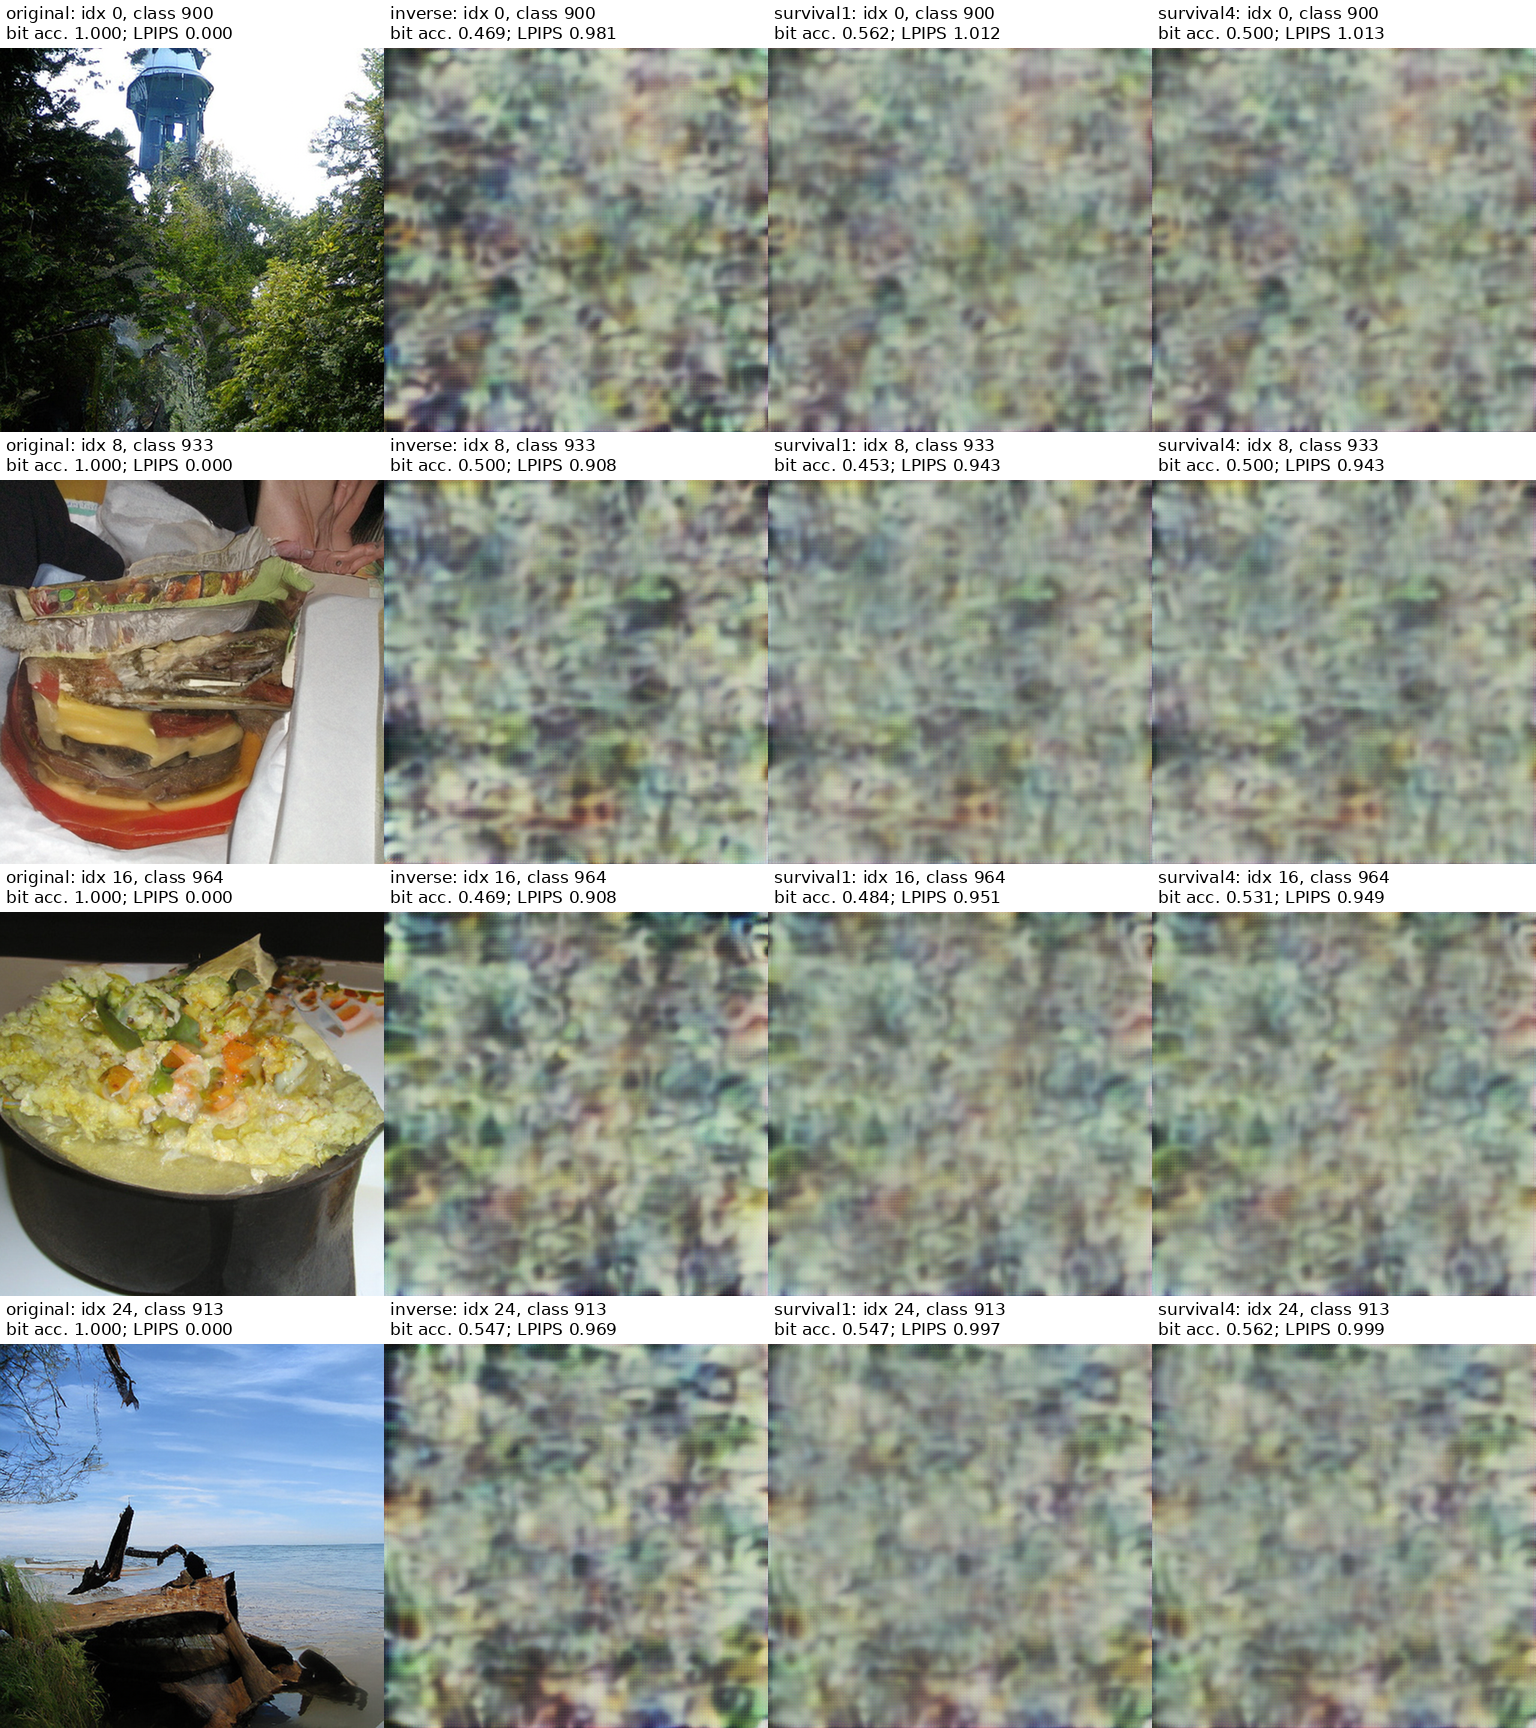
\includegraphics[width=\linewidth]{figures/survival-pilot.png}
\caption{Four coupled pilot examples, one row per original index and one column per candidate. Positions 0, 8, 16 and 24 are displayed without filtering by outcome; this display rule was chosen after the run. Native PNGs remain unchanged. The images expose content failures that detector suppression alone would conceal.}
\end{figure}

The allocation completed in 205 seconds on one H100, including startup and quality evaluation. This development result is retained in the report and compute ledger. It is not evidence of a successful new robust watermark.
